\documentclass{beamer}

\usepackage{../../../latex_style/beamerthemeExecushares}
\usepackage{../../../latex_style/notations}

\title{Session 13: Stochastic gradient descent}
\subtitle{Optimization and Computational Linear Algebra for Data Science}
\author{Léo Miolane}
\date{}

\setcounter{showSlideNumbers}{1}

\begin{document}
\setcounter{showProgressBar}{0}
\setcounter{showSlideNumbers}{0}

\frame{\titlepage}
\setcounter{framenumber}{0}
%\setcounter{showProgressBar}{1}
\setcounter{showSlideNumbers}{1}

\begin{frame}
	\frametitle{Contents}
	\begin{enumerate}
		\item Gradient descent
		\item Convergence analysis for convex functions
		\item Improvements
	\end{enumerate}
\end{frame}

\section{Stochastic gradient descent}

\begin{frame}[t]{Setting}
	\grid

	\vspace{-0.2cm}
	In machine learning, one often has to minimize functions of the form
	$$
	f(x) = \frac{1}{N} \sum_{i=1}^N f_i(x).
	$$
	where $f_i : \R^n \to \R$.

\end{frame}

\begin{frame}[t]{Setting}
	\grid


\end{frame}

\begin{frame}[t]{Stochastic gradient descent}
	\grid
	$$
	f(x) = \frac{1}{N} \sum_{i=1}^N f_i(x).
	$$

	\begin{exampleblock}{}
		Starting at some $x_0 \in \R^n$, perform the updates:
\begin{align*}
	&\text{Pick} \quad i \quad \text{uniformly at random in} \quad \{1, \dots, N\}, \\
	&\text{Update} \quad x_{t+1} = x_t - \alpha_t \nabla f_i(x_t),
\end{align*}
	\end{exampleblock}

\end{frame}

\begin{frame}[t]{Tradeoffs in SGD}
	\grid

	\begin{columns}
		\begin{column}{0.45\textwidth}
			\vspace{-0.5cm}
			\begin{center}
				\textbf{Rapidly decaying step sizes}
			\end{center}
			\hspace*{-0.4cm}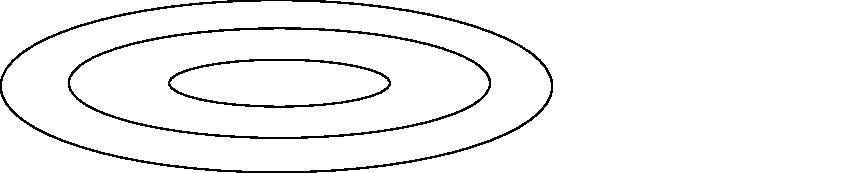
\includegraphics[width=9cm]{../figures/contour.pdf}
			\vspace{7cm}
	\end{column}
	\vrule
		\begin{column}{0.55\textwidth}
			\vspace{-0.5cm}
			\begin{center}
				\textbf{Slowly decaying step sizes}
			\end{center}
			\hspace*{0.4cm}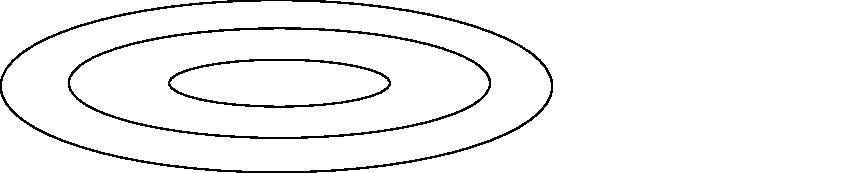
\includegraphics[width=9cm]{../figures/contour.pdf}
			\vspace{7cm}
	\end{column}
	\end{columns}

\end{frame}


\begin{frame}[t]{Convergence analysis}
	\grid

\end{frame}
\begin{frame}[t]{Convergence analysis}
	\grid

\end{frame}
\begin{frame}[t]{GD \ vs \ SGD}
	\grid

	\begin{columns}
		\begin{column}{0.45\textwidth}
			\vspace{-0.5cm}
			\begin{center}
				\textbf{Gradient descent}
			\end{center}
			\vspace{7cm}
	\end{column}
	\vrule
		\begin{column}{0.55\textwidth}
			\vspace{-0.5cm}
			\begin{center}
				\textbf{Stochastic gradient descent}
			\end{center}
			\vspace{7cm}
	\end{column}
	\end{columns}

\end{frame}

\begin{frame}[t]{GD \ vs \ SGD}
	\grid

	\hspace*{-0.7cm}
	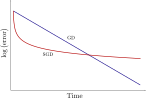
\includegraphics[width=12cm]{../figures/gd_sgd.pdf}

\end{frame}

\appendix
\backupbegin
\begin{frame}[t]
	\frametitle{Questions?}
	\grid

	\pause
\end{frame}
\backupend




\end{document}
